\documentclass[11pt]{article}

\usepackage{fullpage,epsfig,latexsym,picinpar,amsbsy,amsmath,algorithm,mathtools}
\usepackage[noend]{algpseudocode}
\usepackage{xspace}

\usepackage{listings}
\usepackage{color}
\lstset{
  basicstyle=\ttfamily,
  mathescape
}

\lstset{frame=tb,
  language=Java,
  aboveskip=3mm,
  belowskip=3mm,
  showstringspaces=false,
  columns=flexible,
  basicstyle={\small\ttfamily},
  numbers=none,
  numberstyle=\tiny\color{gray},
  keywordstyle=\color{blue},
  commentstyle=\color{dkgreen},
  stringstyle=\color{mauve},
  breaklines=true,
  breakatwhitespace=true,
  tabsize=3
}

\begin{document}

\centerline{\large \bf EE232 Homework 4}
\centerline{Yidi Wang}
\centerline{862114701}

\vskip 0.1in


\paragraph{Question 1} \mbox{} \\
\begin{lstlisting}
R = [2.28125 2.35484 2.57560 2.20767];

cvx_begin
    variables Ic Vc;
    maximize Vc;
    subject to 
        Vc == Ic*sum(R);
        Ic*R(1) <= 3.65;
        Ic*R(2) <= 3.65;
        Ic*R(3) <= 3.65;
        Ic*R(4) <= 3.65;
        Ic >= 0; Ic <= 1.6;
cvx_end
\end{lstlisting}

\noindent
By solving the above convex problem, we can obtain $V_c$ and $I_c$:
\begin{gather*}
    V_c = 13.3486 \, \mathrm{V} \\
    I_c = 1.4171 \, \mathrm{A}
\end{gather*}

%%%%%%%%%%%%%%%%%%%%%%%%%%%%
\paragraph{Question 2} \mbox{} \\
\textbf{Part a} \\
We can obtain the $Y$ matrix according to the transmission network:
$$
Y = 
\begin{bmatrix}
    -20 &  0  &  10 &   0   \\
    0   & -30 &  10 &  10   \\
    10  & 10  & -40 &  10   \\
    0   & 10  & 10  & -20   \\
\end{bmatrix}
$$
\begin{lstlisting}
cvx_begin
    variables $P_1^g$ $P_2^g$ $P_5^g$ $L_2^{ctrl}$ $L_3^{ctrl}$ $L_4^{ctrl}$ $\theta_2$ $\theta_3$ $\theta_4$ $\theta_5
    $
    minimize $ \sum_{h=1}^{10} \big( C_{1,h}(P_1^g) + C_{2,h}(P_2^g) + C_{5,h}(P_5^g) \big) $
    subject to
        $ 1.5 \leq P_1^g \leq 5; \; 1.5 \leq P_2^g \leq 5; \; 1.5 \leq P_5^g \leq 5; $
        
        $ P_1^g + P_2^g + P_5^g == L_2^{ctrl} + L_3^{ctrl} + L_4^{ctrl} + L_2^{fixed} + L_3^{fixed} + L_4^{fixed} $

        $ L_2^{ctrl} \geq 0; \; L_3^{ctrl} \geq 0; \; L_4^{ctrl} \geq 0 $

        $
        \sum_{h=1}^{10} L_{2,h}^{ctrl} == 10;   \;
        \sum_{h=3}^{9} L_{3,h}^{ctrl} == 12;    \;
        \sum_{h=2}^{6} L_{4,h}^{ctrl} == 7;
        $

        $ L_{2,h}^{ctrl} == 0; $
        $ L_{3,h}^{ctrl} == 0 \; (h < 3, h > 9); $
        $ L_{4,h}^{ctrl} == 0 \; (h < 2, h > 6); $
        
        $
        \begin{bmatrix}
            P_2^g - L_2^{ctrl} - L_2^{fixed}    \\
            - L_3^{ctrl} - L_3^{fixed}          \\
            - L_4^{ctrl} - L_4^{fixed}          \\
            P_5^g                       
        \end{bmatrix}
        =
        [Y]
        \begin{bmatrix}
            \theta_2    \\
            \theta_3    \\
            \theta_4    \\
            \theta_5
        \end{bmatrix}
        $
cvx_end
\end{lstlisting}

\begin{figure}[H]
    \centering
    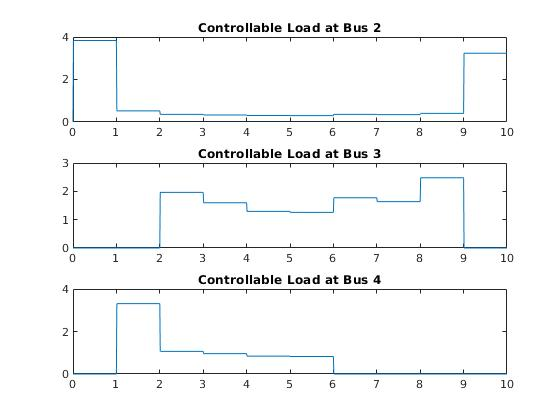
\includegraphics[scale=0.6]{figs/q2_a.jpg}
    \caption{Schedule of controllable load with infinite transmission line capacity}
    \label{fig::q2a}
\end{figure}

\noindent
\textbf{Part b} \\
\begin{lstlisting}
cvx_begin
    variables $P_1^g$ $P_2^g$ $P_5^g$ $L_2^{ctrl}$ $L_3^{ctrl}$ $L_4^{ctrl}$ $\theta_2$ $\theta_3$ $\theta_4$ $\theta_5
    $
    minimize $ \sum_{h=1}^{10} \big( C_{1,h}(P_1^g) + C_{2,h}(P_2^g) + C_{5,h}(P_5^g) \big) $
    subject to
        $ 1.5 \leq P_1^g \leq 5; \; 1.5 \leq P_2^g \leq 5; \; 1.5 \leq P_5^g \leq 5; $

        $ P_1^g + P_2^g + P_5^g == L_2^{ctrl} + L_3^{ctrl} + L_4^{ctrl} + L_2^{fixed} + L_3^{fixed} + L_4^{fixed} $

        $ L_2^{ctrl} \geq 0; \; L_3^{ctrl} \geq 0; \; L_4^{ctrl} \geq 0 $

        $
        \sum_{h=1}^{10} L_{2,h}^{ctrl} == 10;   \;
        \sum_{h=3}^{9} L_{3,h}^{ctrl} == 12;    \;
        \sum_{h=2}^{6} L_{4,h}^{ctrl} == 7;
        $

        $ L_{2,h}^{ctrl} == 0; $
        $ L_{3,h}^{ctrl} == 0 \; (h < 3, h > 9); $
        $ L_{4,h}^{ctrl} == 0 \; (h < 2, h > 6); $
        
        $
        \begin{bmatrix}
            P_2^g - L_2^{ctrl} - L_2^{fixed}    \\
            - L_3^{ctrl} - L_3^{fixed}          \\
            - L_4^{ctrl} - L_4^{fixed}          \\
            P_5^g                       
        \end{bmatrix}
        =
        [Y] \cdot
        \begin{bmatrix}
            \theta_2    \\
            \theta_3    \\
            \theta_4    \\
            \theta_5
        \end{bmatrix}
        $

        $ | 10 \cdot (-\theta_3) | \leq 1.5 $
        $ | 10 \cdot (\theta_2 - \theta_4) | \leq 1.5 $
cvx_end
\end{lstlisting}

\begin{figure}[H]
    \centering
    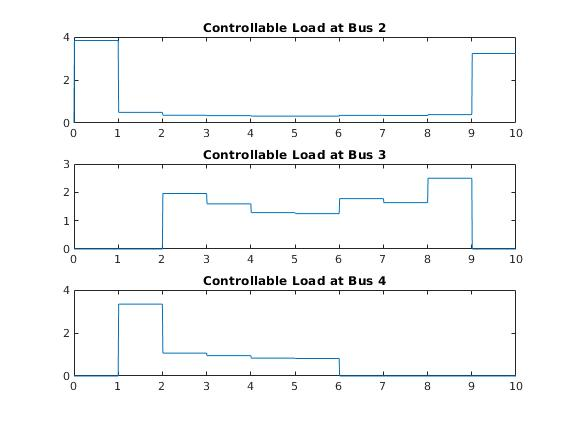
\includegraphics[scale=0.6]{figs/q2_b.jpg}
    \caption{Schedule of controllable load with limited transmission line capacity}
    \label{fig::q2b}
\end{figure}

\noindent
\textbf{Part c} \\
Optimal generation cost in (a): \$49377 \\
Optimal generation cost in (b): \$49377 \\
PAR (controllable) in (a): 1.3172   \\
PAR (controllable) in (b): 1.3172   \\
PAR (total) in (a): 1  \\
PAR (total) in (b): 1

\pagebreak
%%%%%%%%%%%%%%%%%%%%%%%%%%%%
\paragraph{Question 3} \mbox{} \\
\begin{lstlisting}
cvx_begin
    variables $P_1^g$ $P_2^g$ $P_5^g$ $L_2^{ctrl}$ $L_3^{ctrl}$ $L_4^{ctrl}$ $\theta_2$ $\theta_3$ $\theta_4$ $\theta_5
    $
    minimize $ \sum_{h=1}^{10} \big( L_{2,h}^{fixed} + L_{3,h}^{fixed} + L_{4,h}^{fixed} + L_{2,h}^{ctrl} + L_{3,h}^{ctrl} + L_{4,h}^{ctrl} \big) \times Price_h $
    subject to
        $ 1.5 \leq P_1^g \leq 5; \; 1.5 \leq P_2^g \leq 5; \; 1.5 \leq P_5^g \leq 5; $
        
        $ P_1^g + P_2^g + P_5^g == L_2^{ctrl} + L_3^{ctrl} + L_4^{ctrl} + L_2^{fixed} + L_3^{fixed} + L_4^{fixed} $

        $ L_2^{ctrl} \geq 0; \; L_3^{ctrl} \geq 0; \; L_4^{ctrl} \geq 0 $

        $
        \sum_{h=1}^{10} L_{2,h}^{ctrl} == 10;   \;
        \sum_{h=3}^{9} L_{3,h}^{ctrl} == 12;    \;
        \sum_{h=2}^{6} L_{4,h}^{ctrl} == 7;
        $

        $ L_{2,h}^{ctrl} == 0; $
        $ L_{3,h}^{ctrl} == 0 \; (h < 3, h > 9); $
        $ L_{4,h}^{ctrl} == 0 \; (h < 2, h > 6); $
        
        $
        \begin{bmatrix}
            P_2^g - L_2^{ctrl} - L_2^{fixed}    \\
            - L_3^{ctrl} - L_3^{fixed}          \\
            - L_4^{ctrl} - L_4^{fixed}          \\
            P_5^g                       
        \end{bmatrix}
        =
        [Y]
        \begin{bmatrix}
            \theta_2    \\
            \theta_3    \\
            \theta_4    \\
            \theta_5
        \end{bmatrix}
        $
cvx_end
\end{lstlisting}

\begin{figure}[H]
    \centering
    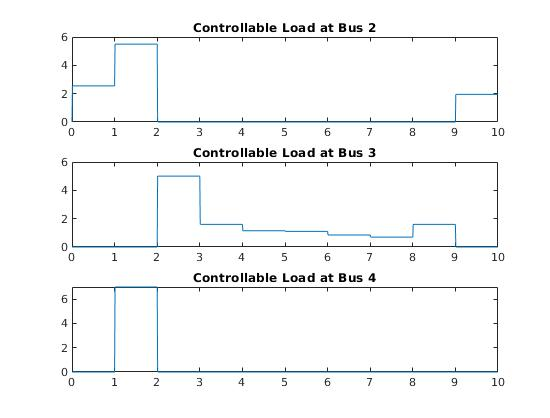
\includegraphics[scale=0.6]{figs/q3.jpg}
    \caption{Schedule of controllable load with different hourly price}
    \label{fig::q3}
\end{figure}

\noindent
Optimal price: \$2187   \\
PAR (controllable) in this case: 1.3172    \\
PAR (total) in this case: 2.4978    \\ 
This is not desirable. PAR is far from 1, which means that the load is not stable.


%%%%%%%%%%%%%%%%%%%%%%%%%%%%
\paragraph{Question 4} \mbox{} \\
\begin{lstlisting}
cvx_begin
    variables $P_1^g$ $P_2^g$ $P_5^g$ $L_2^{ctrl}$ $L_3^{ctrl}$ $L_4^{ctrl}$ $\theta_2$ $\theta_3$ $\theta_4$ $\theta_5
    $
    minimize $ \sum_{h=1}^{10} \big( L_{2,h}^{fixed} + L_{3,h}^{fixed} + L_{4,h}^{fixed} + L_{2,h}^{ctrl} + L_{3,h}^{ctrl} + L_{4,h}^{ctrl} \big) \times 40 $
            $+ \max\big( L_{2,h}^{fixed} + L_{3,h}^{fixed} + L_{4,h}^{fixed} + L_{2,h}^{ctrl} + L_{3,h}^{ctrl} + L_{4,h}^{ctrl} \big) \times 80
    $
    subject to
        $ 1.5 \leq P_1^g \leq 5; \; 1.5 \leq P_2^g \leq 5; \; 1.5 \leq P_5^g \leq 5; $
        
        $ P_1^g + P_2^g + P_5^g == L_2^{ctrl} + L_3^{ctrl} + L_4^{ctrl} + L_2^{fixed} + L_3^{fixed} + L_4^{fixed} $

        $ L_2^{ctrl} \geq 0; \; L_3^{ctrl} \geq 0; \; L_4^{ctrl} \geq 0 $

        $
        \sum_{h=1}^{10} L_{2,h}^{ctrl} == 10;   \;
        \sum_{h=3}^{9} L_{3,h}^{ctrl} == 12;    \;
        \sum_{h=2}^{6} L_{4,h}^{ctrl} == 7;
        $

        $ L_{2,h}^{ctrl} == 0; $
        $ L_{3,h}^{ctrl} == 0 \; (h < 3, h > 9); $
        $ L_{4,h}^{ctrl} == 0 \; (h < 2, h > 6); $
        
        $
        \begin{bmatrix}
            P_2^g - L_2^{ctrl} - L_2^{fixed}    \\
            - L_3^{ctrl} - L_3^{fixed}          \\
            - L_4^{ctrl} - L_4^{fixed}          \\
            P_5^g                       
        \end{bmatrix}
        =
        [Y]
        \begin{bmatrix}
            \theta_2    \\
            \theta_3    \\
            \theta_4    \\
            \theta_5
        \end{bmatrix}
        $
cvx_end
\end{lstlisting}

\begin{figure}[H]
    \centering
    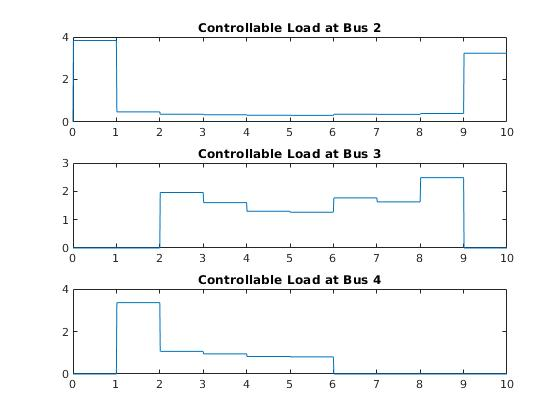
\includegraphics[scale=0.6]{figs/q4.jpg}
    \caption{Schedule of controllable load with energy and power charge}
    \label{fig::q4}
\end{figure}

\noindent
Optimal price: \$2776.8   \\
PAR (controllable) in this case: 1.3172    \\
PAR (total) in this case: 1


%%%%%%%%%%%%%%%%%%%%%%%%%%%%
\pagebreak
\paragraph{Question 5} \mbox{} \\
\textbf{Part a, b} \\
\begin{figure}[H]
    \centering
    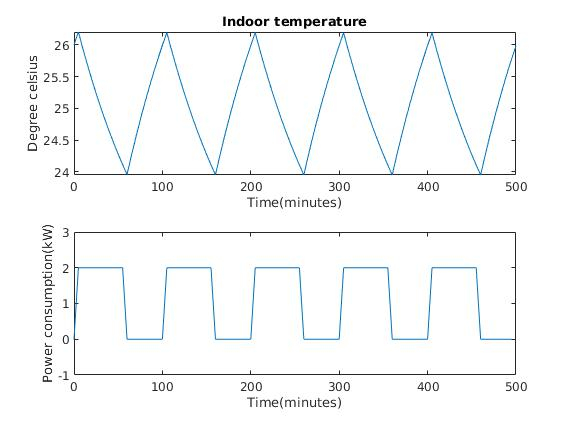
\includegraphics[scale=0.5]{figs/q5_a.jpg}
    \caption{Indoor temperature and power consumption}
    \label{fig::q5a}
\end{figure}

Total energy usage: 9.1667 kWh

\noindent
\textbf{Part c} \\
\begin{figure}[H]
    \centering
    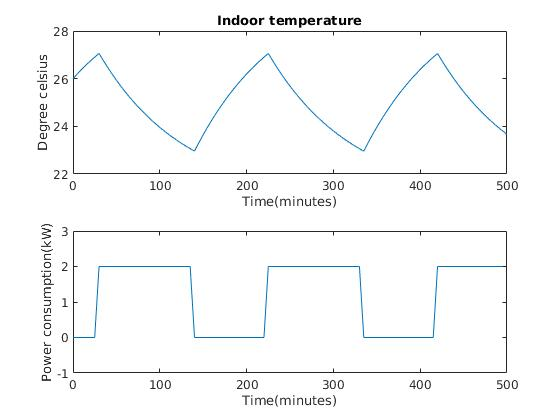
\includegraphics[scale=0.5]{figs/q5_c.jpg}
    \caption{Indoor temperature and power consumption}
    \label{fig::q5c}
\end{figure}

Total energy usage: 10 kWh

\end{document}

